\section{Infrastructure Setup}
We identify four main services which require machine-to-machine communication and, thus, are susceptible to the firewall rules that we'll define:\\
\begin{itemize}
\item an \textbf{Apache} web server reachable through \textbf{TCP} ports \textbf{80} (HTTP) and \textbf{443} (HTTPS) at \textbf{100.100.6.2};
\item a \textbf{DNS service} reachable through standard \textbf{UDP} port \textbf{53} at \textbf{100.100.1.2};
\item a \textbf{rsyslog at logserver} which we will make reachable through standard \textbf{UDP} port \textbf{514} at \textbf{100.100.1.3};
\item a \textbf{proxy server} reachable through port \textbf{3128} at \textbf{100.100.6.3}, to be configured later on Assignemnt 3.
\end{itemize}

We thus identify two new subnetworks: the \textbf{Internal Servers} subnetwork \textbf{100.100.1.0$/$24} and the \textbf{DMZ} subnetwork \textbf{100.100.6.0$/$24}, and for the sake of defining the scope of this assignment and the setup of the whole infrastructure, we should also consider two additional details:\\
\begin{itemize}
\item One of the four services - web server - is already setup and running in the system: it does not need to be configured or launched;
\item the \textbf{proxy server} is to be configured on the next assignment: for now, knowing from the \textbf{zentyal} portal that it is provided on port 3128 is enough.
\end{itemize}

This leaves us with the only \textbf{DNS service} to be configured at the moment, and the \textbf{rsyslog} process at \textbf{logserver} and at each of its clients to be defined later. The first step has been performed by following the instructions provided with the assignment: by accessing the \textbf{zentyal} portal at \textbf{100.100.1.2} on port \textbf{8843} - credentials have been changed - we added as forwarders the suggested IP addresses and specified the domain name - \textbf{acme.group27}. Then, the file located at \textbf{$/$etc$/$zentyal$/$dns.conf} on the aforementioned machine was modified including the target subnetworks (Clients and DMZ, that are the ones which will exploit the service).\\
At this point, pairs of IP addresses and hostnames were specified in the portal, so that the well-known machines of the network can now be associated with the following names:\\
\begin{itemize}
\item \textbf{kali}.acme.group27;
\item \textbf{watchdog}.acme.group27;
\item \textbf{dc}.acme.group27;
\item \textbf{web}.acme.group27;
\item \textbf{proxy}.acme.group27;
\item \textbf{coffee}.acme.group27;
\end{itemize}

also, as suggested in the assignment, the external services machines were provided with an external DNS service such as 8.8.8.8 in their DHCPv4 configuration. Please notice also that the \textit{logserver} was not given a name since it is only meant to be accessed by the SPOCK environment or by SSH and is not offering any browser-related service - and the same reasoning could be applied to the first two machines, \textit{kali} and \textit{arpwatch}, which we could exclude from this pairing list.\\
Last step was to actually modify the \tetxbf{DHCPv4} settings in the two main routers to set the \textbf{dc} machine as the \textbf{DNS server} in the Internal Servers network, after having disabled the \textbf{Service Unbound DNS} in both routers.\\
Keep also in mind that some of the machines with predefined IP addresses (fixed, not assigned by DHCP service) had either to be configured externally, or had to have their \textit{$/$etc$/$resolv.conf} file re-configured by modifying the IP address of their nameserver (for instance, Proxy and Kali machines).\\
The \textbf{DNS service} configuration is tested in section 5.

\subsection{Log server}
The \textbf{rsyslog} service at \textbf{logserver} was configured by modifying the file \textit{$/$etc$/$rsyslog.conf}, whose lines about \textbf{UDP} remote service were uncommented so that the service is listening on UDP port \textbf{514} (for further details on this, see the last paragraph) for log messages to record from its clients. Then, a \textbf{template} was defined in this config file, so that for every log message that is received, the service records it under path \textit{$/$var$/$log$/$machine$/$process.log} - e.g., when process \textbf{login} from \textbf{webserver} machine sends a log message to the \textbf{logserver}, it is recorded under $/$webserver$/$login.log under the logging directory.\\
Then, for each \textbf{client} of the service, the very same config file was modified - so for every machine on \textbf{DMZ} and \textbf{Internal Servers} subnetworks, by appending to the end of the file \textit{*.* @100.100.1.3:514} to specify that each log message from every process of the machine must be sent to the \textbf{logserver} through \textbf{UDP} protocol on port \textbf{514}. Figures \textbf{1} and \textbf{2} at page 8 show the outcome of this configuration.\\

\begin{figure}[H]
\centering
\begin{minipage}{.5\textwidth}
  \centering
  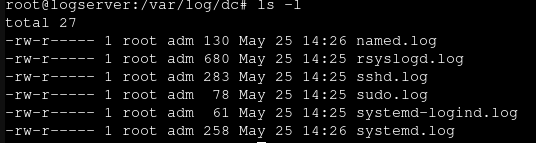
\includegraphics[width=1\textwidth]{logserver_dc.png}
  \caption[a]{Log files sent by 100.100.1.2 - dc machine.}\label{fig:1}
\end{minipage}%
\begin{minipage}{.5\textwidth}
  \centering
  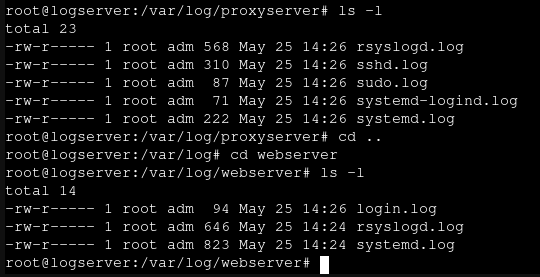
\includegraphics[width=1\textwidth]{logserver_dmz.png}
  \caption[a]{log files sent by machines in DMZ subnet.}\label{fig:2}
\end{minipage}
\end{figure}
